\documentclass[a4paper]{article}
\usepackage{polski}
\usepackage[utf8]{inputenc}
\usepackage{graphicx} 
\usepackage{wrapfig} 


\title{Matematyka ?}
\author{Bartosz Mazurkiewicz}
\begin{document}
\maketitle
\noindent
\begin{thebibliography}{2}

\bibitem{cewe2008}
  Alicja Cewe,
  \emph{Tablice Matematyczne}.
Podkowa
2008.

\bibitem{oetiker2007}
  Tobias Oetiker,
  \emph{Nie za krótkie wprowadzenie do systemu LATEX }.
Wydanie drugie, poprawione, uaktualnione i rozszerzone
Styczeń 2007.
\end{thebibliography}

\paragraph{Odsyłacze:} 

Obrazek : \ref{obrazek} na stronie~\pageref{obrazek}.\\
Wzór na równanie kwadratowe : \ref{wzór} na stronie~\pageref{wzór}. \\
Tabliczka mnożenia : \ref{tabmno} na stronie~\pageref{tabmno}. \\
Tablica kątów : \ref{tabkat} na stronie~\pageref{tabkat}. \\


\section{Figury i Rówanie kwadratowe}
\subsection{Jak wyglądają figury płaskie: }
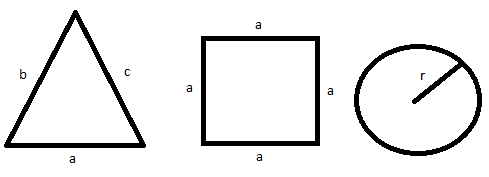
\includegraphics[width=2in]{k} \label{obrazek}
	\subsection{Pola i Obwody kilku figur płaskich}

\begin{enumerate}
	\item Kwadrat
		\begin{itemize}
			\item pole : $a^{2}$ 
			\item obwód : 4a 
		\end{itemize}
	\item Trójkąt
		\begin{itemize}
			\item pole : $\frac{a*h}{2}$ 
			\item obwód : $a+b+c$ 
			\item pole trójkąta równobocznego : $\frac{a^{2}\sqrt{3}}{4}$ 
		\end{itemize} 			
	\item Koło
		\begin{itemize}
			\item pole : $\pi r^{2}$ 
			\item obwód  $2\pi r$ 
		\end{itemize}
\end{enumerate}

\subsection{Pola i Objętości figur obrotowych}
\begin{enumerate}
	\item Walec
		\begin{itemize}
			\item pole : 2Pp+Pb=$2\pi r^{2}+2\pi rh$ 
			\item objętość : $\pi r^{2}H$ 
		\end{itemize}
	\item Stożek
		\begin{itemize}
			\item pole : Pp+Pb=$\pi r^{2}+\pi rl$ 
			\item objętość : $\frac{1}{3}\pi r^{2}H$ 
		\end{itemize} 			
	\item Kula
		\begin{itemize}
			\item pole : $4\pi r^{2}$ 
			\item objętość :  $\frac{4}{3}\pi r^{3}$ 
		\end{itemize}
\end{enumerate}
\subsection{Równanie kwadratowe}
y=$ax^{2}+bx+c$
\label{wzór}












\section{Podstawowe tablice używane w matematyce}
	

	\subsection{Tabliczka mnożenia}	

	\begin{tabular}{|c|c|c|c|c|c|c|c|c|c|c|}

 \hline 
	 X & 1 & 2 & 3 & 4 & 5 & 6 & 7 & 8 & 9 & 10 \\
 \hline 
 	1 & 1 & 2 & 3 & 4 & 5 & 6 & 7 & 8 & 9 & 10 \\
 \hline 
	2 & 2 & 4 & 6 & 8 & 10 & 12 & 14 & 16 & 18 & 20 \\
\hline 
 	3 & 3 & 6 & 9 & 12 & 15 & 18 & 21 & 24 & 27 & 30 \\
\hline 
 	4 & 4 & 8 & 12 & 16 & 20 & 24 & 28 & 32 & 36 & 40 \\
\hline 
 	5 & 5 & 10 & 15 & 20 & 25 & 30 & 35 & 40 & 45 & 50 \\
\hline 
 	6 & 6 & 12 & 18 & 24 & 30 & 36 & 42 & 48 & 54 & 60 \\
\hline 
 	7 & 7 & 14 & 21 & 28 & 35 & 42 & 49 & 56 & 63 & 70 \\
\hline 
 	8 & 8 & 16 & 24 & 32 & 40 & 48 & 56 & 64 & 72 & 80 \\
\hline 
 	9 & 9 & 18 & 27 & 36 & 45 & 54 & 63 & 72 & 81 & 90 \\
\hline 
 	10 & 10 & 20 & 30 & 40 & 50 & 60 & 70 & 80 & 90 & 100 \\
\hline 
\end{tabular} 
\label{tabmno}


	\subsection{Tablica z podstawowymi kątami}	
	\begin{tabular}{|c|c|c|c|c|c|}
 \hline 
	$\alpha$ & $0^{\circ}$ & $30^{\circ}$ & $45^{\circ}$ & $60^{\circ}$ & $90^{\circ}$  \\
 \hline 
 	sin $\alpha$ & 0 &  $\frac{1}{2}$ &  $\frac{\sqrt{2}}{2}$ & $\frac{\sqrt{3}}{2}$ & 1 \\
 \hline 
	cos $\alpha$ & 1 &  $\frac{\sqrt{3}}{2}$ &  $\frac{\sqrt{2}}{2}$ &  $\frac{1}{2}$  & 0  \\
\hline 
 	tan $\alpha$ & 0 &  $\frac{\sqrt{3}}{3}$ & 1 & $\sqrt{3}$ & -  \\
\hline 
 	ctg $\alpha$ & - & $\sqrt{3}$ & 1 &  $\frac{\sqrt{3}}{3}$ & 0  \\

\hline 
\end{tabular}
\label{tabkat}


\end{document}